%
% CHAPTER Versuch 1
%
\chapter{Programmierung der AD/DA-Wandlerkarte}
\label{chap:VERSUCH_1}

\section{Fragestellung, Messprinzip, Aufbau, Messmittel}
\label{chap:VERSUCH_1_FRAGESTELLUNG}
Fragestellung: Die AD/DA-Wandlerkarte des ME-RedLab USB-1208LS soll mit einem Python-Skript programmiert und getestet werden.\\
Messprinzip: Anhand eines Python-Skriptes sollen eine Reihe von unterschiedlichen Werten aus der AD/DA-Wandlerkarte des ME-RedLab USB-1208LS ausgelesen und grafisch dargestellt werden. Dieses Skript soll anschließend um eine Funktion erweitert werden, die eine Konsoleneingabe auf der AD/DA-Wandlerkarte ausgibt.\\
Aufbau: Für den Versuch wird eine Multifunktionsbox ME-RedLab USB-1208LS verwendet. Diese besitzt mehrere analoge und digitale Ein-/Ausgänge. Für die Eingangsspannungsbereich wird der single-ended-Modus und eine Spannung von $\pm$10 V verwendet, für den Ausgangsspannungsbereich 0 bis 5 V. Die Board Configuration ist auf 8 single-ended channels einzustellen.\\
Messmittel: ME-RedLab USB-1208LS

\section{Messwerte}
\label{chap:VERSUCH_1_MESSWERTE}
Das Python-Skript ergab die folgende Darstellung der ausgelesenen Werte:
\begin{figure}[H]
\begin{center}
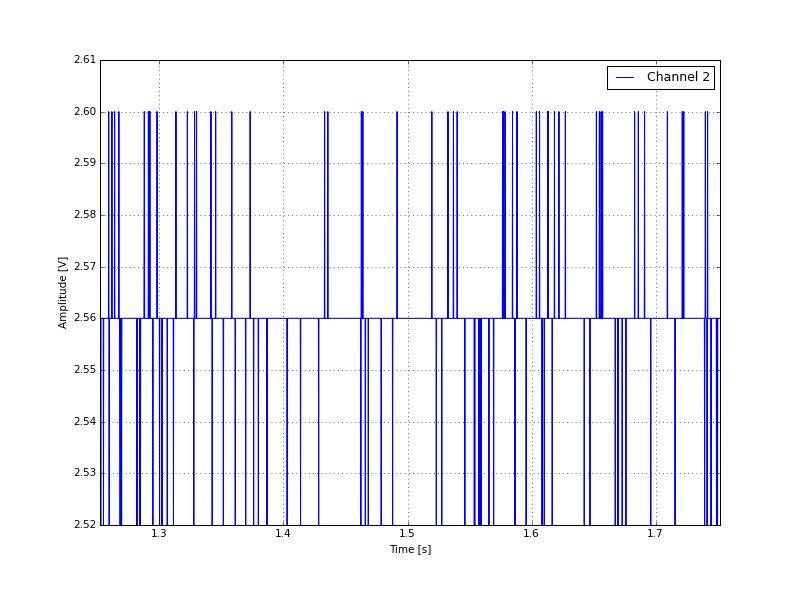
\includegraphics[scale=0.65]{output.png}
\caption{Ausgelesene Werte der ME-RedLab USB-1208LS}
\end{center}
\end{figure}

\section{Auswertung}
\label{chap:VERSUCH_1_AUSWERTUNG}
Das Bild zeigt mehrere markante Spitzen sowohl nach oben als auch nach unten.

\section{Interpretation}
\label{chap:VERSUCH_1_INTERPRETATION}
Bei den Spitzen handelt es sich um Quantisierungsfehler.